\section{ Vorausberechnung der Schaltung}

Folgende Eigenschaften der Filter sind in häuslicher Vorarbeit zu bestimmen und zum Praktikumstermin vorzulegen:
\subsection{Grundverstärkung und Grenzfrequenzen der Hoch- und Tiefpässe }
\subsection{Mittenfrequenz und Bandbreite des Bandpasses }
\subsection{Sperrfrequenz der Bandsperre }
\subsection{Übertragungsfunktionen mit Matlab symbolisch berechnet }
\subsection{Übertragungsfunktionen (Betrag und Phase) mit Matlab numerisch berechnet} 
\subsection{Spice Simulationsergebnisse für das Frequenzverhalten (AC-Analyse)}

Die Eigenschaften 1-3) können entweder berechnet (siehe Abschnitte 6 und 7) oder aus Simulationen mit Spice (z.B. PSpice oder LTSpice) entnommen werden. Der Berechnungsgang bzw. Schaltung und Plot der Spice-Simulation sind zum Labortermin vorzulegen und in das Protokoll mit aufzunehmen, genauso wie der Matlab-Code.


\subsection{Aufbau}

% grafik einbinden
\begin{figure}[H]
    \begin{center}
        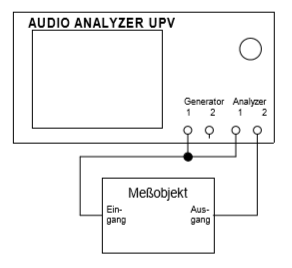
\includegraphics[width=0.5\textwidth]{img/Blockschalt.PNG}
        \caption{Blockschaltbild, Quelle: "GNP3 Aktive RC-Filter.pdf" }
        \label{fig:A2_label}
    \end{center}
\end{figure}

%%%%%%%%%%%%%%%%%%%%%%%%%%%%%%%%%%%%%%%%%%%%%%%%Comments
%zu 2 :Formeln bzw. Spice-Plots und Ergebnisse der Vorausberechnung für Grundverstärkung und Grenzfrequenzen der Hoch- und Tiefpässe, Mittenfrequenz und Bandbreite des Bandpasses, Sperrfrequenz der Bandsperre. 